% Dokumentace projektu GAL 2014
% Vendula Poncová, xponco00
% Alena Chernikava, xcerni07

\documentclass[a4paper, 12pt, titlepage, final]{article}[3. prosinec 2011]

\newcommand{\uv}[1]{\quotedblbase #1\textquotedblleft}
\newcommand{\mensi}{$<$}
\newcommand{\vetsi}{$>$}

\usepackage[left=2.5cm,text={16cm, 25cm},top=2cm]{geometry}
\usepackage[czech]{babel}
\usepackage[utf8]{inputenc}
\usepackage[IL2]{fontenc}
\usepackage[dvipdf]{graphicx}
\usepackage{color}

\newcommand{\url}[1]{\textit{#1}}
\begin{document}

%%%%%%%%%%%%%%%%%%%%%%%%%%%%%%%%%%%%%%%%%%%%%%%%%%%%%%%%%%%%%%%%%%%%%%%%%
% titulni strana - DON'T TOUCH! MAGIC!

\begin{titlepage}
\begin{center}

\textsc{
\Large Fakulta informačních technologií 
\medskip\\
Vysoké učení technické v~Brně}

\vspace{\stretch{0.190}}

{\parbox{5cm}{\centering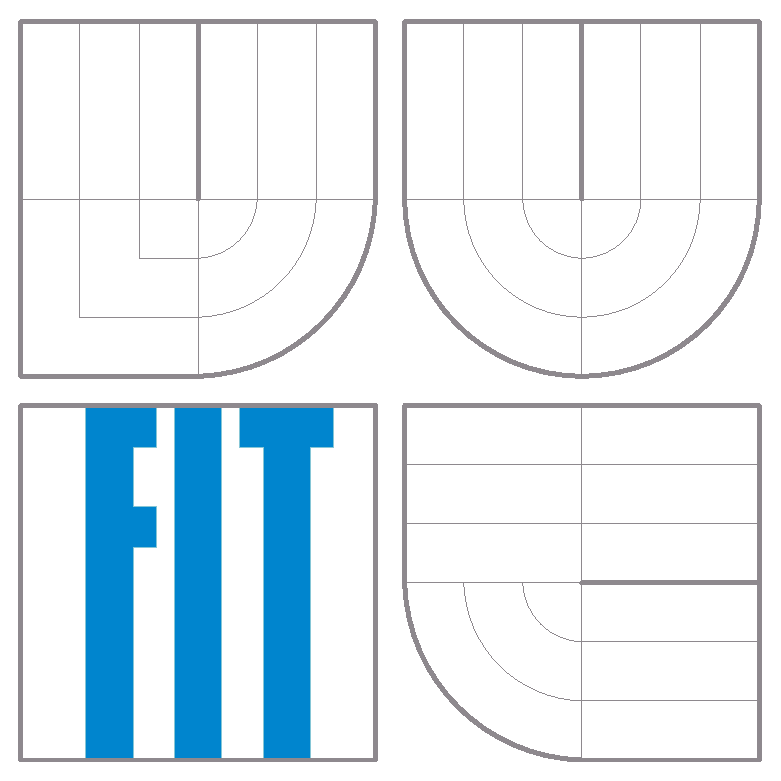
\includegraphics[height=5cm]{img/logo.eps}}}

\vspace{\stretch{0.190}}

{\large Dokumentace projektu do předmětu GAL} \medskip \\
{\LARGE Paralelizace Egerváryho algoritmu} 


\vspace{\stretch{0.618}}

\end{center}

{\large
Tým 33

Vendula Poncová (\texttt{xponco00})

Alena Chernikava (\texttt{xcerni07})
} \hfill {\large\today}

\end{titlepage}

%%%%%%%%%%%%%%%%%%%%%%%%%%%%%%%%%%%%%%%%%%%%%%%%%%%%%%%%%%%%%%%%%%%%%%%%%
% text dokumentace

\pagenumbering{arabic}
\setcounter{page}{1}

%------------------------------------------------------------------------
\section{Úvod}

V této dokumentaci popisujeme návrh a implementaci sekvenční a paralelní varianty Egerváryho algoritmu. S oběmi implementacemi jsme provedly experimenty pro různé vstupní grafy a různé počty procesů. V závěru shrnujeme naše výsledky a porovnáváme je s teoretickými poznatky.

%------------------------------------------------------------------------
\section{Egerváryho algoritmus}

Egerváryho algoritmus umožňuje vypočítat maximální párování v neorientovaném bipartitním grafu. V této kapitole popisujeme, jak algoritmus funguje a jak jsme jej naimplementovaly. Sekvenční variantu Egerváryho algoritmu jsme převzaly z knihy Graph Theory[\cite{Bondy:2008}]. Snažily jsme se najít i jiný zdroj, ale uvedený algoritmus se vždy odlišoval. Z téhož důvodu se nám nepodařilo najít odpovídající paralelní variantu, a proto jsme navrhly vlastní.

\subsection{Maximální párování}

Párování \textit{M} je množina po dvou nesousedících hran grafu \textit{G=(V,E)}. Říkáme, že vrchol \textit{v} je pokrytý \textit{M}, jestliže \textit{v} je incidenční s hranou v \textit{M}. Potom \textit{M} je maximální, jestliže pokrývá co nejvíce vrcholů grafu \textit{G}. Problém nalezení maximálního párování lze definovat následovně: Pro graf \textit{G} najděte maximální párování \textit{M} v \textit{G}. 

Egerváryho algoritmus tento problém řeší pomocí Bergésova teorému, který říká, že párování \textit{M} v grafu \textit{G} je maximální tehdy a jen tehdy, když \textit{G} neobsahuje \textit{M-augmenting path}. \textit{M-augmenting path} je cesta v \textit{G}, jejíž hrany jsou střídavě v \textit{M} a v \textit{E/M} a počáteční a koncový vrchol není pokrytý \textit{M}. Na této cestě pak lze upravit \textit{M} tak, že hrany, které patřily do \textit{M}, tam již patřit nebudou, a hrany, které nepatřily do \textit{M}, tam patřit budou. Tím se počet vrcholů pokrytých \textit{M} zvýší o jedna.

%Efektivní způsob, jak takovou cestu najít, je budování stromu, jehož kořenem je uzel, který není pokrytý M,

TODO : dopsat

%------------------------------------------------------------------------
\subsection{Sekvenční verze algoritmu}

\subsubsection*{Návrh}

Sekvenční variantu jsme zachovaly v podobě, v jaké ji popisujeme v předcházející kapitole. Zbývalo vhodně zvolit datové struktury. 

Graf jsme se rozhodly reprezentovat seznamem následníků. Egerváryho algoritmus pracuje s neorientovanými grafy a s atributy na hranách. Proto seznam následníků obsahuje hrany pro oba směry a hrany obsahují odkazy na své protějšky.

Dále bylo třeba navrhnout efektivní datovou strukturu pro strom. Algoritmus vyžaduje, aby se stromem dalo projít od listu ke kořeni, aby strom mohl být vyloučen z grafu, jestliže se jedná o \textit{APS-tree}, a aby bylo možné do stromu přidávat uzly a všechny je zase odebrat, jestliže se našla \textit{M-augmenting path}. 

Z těcho důvodů jsme se rozhodly stromy reprezentovat jako seznam stromů, jejichž atributy jsou status a kořen stromu. Stromy, které se vyhodnotily jako \textit{APS-tree} budou mít status \texttt{APSTREE}, stromy, ve kterých se nalezla \textit{M-augmenting path} budou mít status \texttt{NONE} a konečně strom, který je právě zpracovávaný bude mít status \texttt{ACTUAL}. Každý uzel pak obsahuje atribut ukazatel na strom a ukazatel na vstupní hranu.

Časové složitosti požadovaných operací jsou pak následující: Stromem lze projít od listu ke kořeni v lineárním čase závislém na výšce stromu. Strom lze vyloučit z grafu v konstatním čase nastavením statusu na \texttt{APSTREE}. Do stromu lze přidat uzel v konstatním čase nastavením ukazatele na strom ve struktuže uzlu. Ze stromu lze odebrat všechny uzly v konstatním čase nastavením statusu stromu na \texttt{NONE}.

\subsubsection*{Implementace}

%------------------------------------------------------------------------
\subsection{Paralelní verze algoritmu}

\subsubsection*{Návrh}

Vycházely jsme ze sekvenční podoby Egerváryho algoritmu. Při hledaní \textit{M-alternating path} se vytváří strom, který je podgrafem vstupního grafu. Po nalezení cesty, případně \textit{APS-tree}, se pak provádí změny v grafu právě v rámci vytvořeného stromu. Na jiné uzly a hrany změny nemají žádný vliv. Graf by proto mohl být zpracováván více procesy, pokud by procesy vytvářely navzájem disjuktní stromy. Otázkou pak zůstává, jak zajistit, aby stromy byly disjuktní. V ideálním případě, uzel, o který má proces zájem, do žádného stromu nepatří. Proces pak může tento uzel připojit ke svému stromu. Pokud uzel již patří do stromu jiného procesu, dochází ke konfliktu. V Egerváryho algoritmu může dojít ke čtyřem typům takových konfliktů: \textit{R-R}, \textit{R-B}, \textit{B-B}, \textit{B-R}. Konflikt typu \textit{R-B} znamená, že proces chce z uzlu typu \texttt{RED} přejít na uzel jiného stromu typu \texttt{BLUE}. Analogicky pro ostatní typy.

Typy konfliktů jsou znázorněné na obrázku (OBRÁZEK). Z obrázku jsou zřejmé následující tvrzení: pokud došlo ke konfliktu typu \textit{R-R} nebo \textit{B-B}, pak jsme našli \textit{M-alternating path} z kořenu jednoho stromu do kořenu druhého stromu. Pokud došlo ke konfliktu typu \textit{R-B}, pak podstrom z uzlu \textit{R}, je součástí druhého stromu. Pokud došlo ke konfliktu typu \textit{B-R}, pak z uzlu \textit{B} vychází více hran, které patří do \textit{M}, což znamená, že \textit{M} není párování. Pokud algoritmus pracuje správně, tak by k takovému konfliktu nikdy nemělo dojít. 

Ve dvou případech se tedy výpočet pravděpodobně urychlí. V jednom případě bude třeba jeden strom zahodit a jeho část přiřadit druhému stromu. Pokud ale uvážíme nejhorší možný případ, pak může docházet k tomu, že než se proces dopracuje k nějakému výsledku, bude jiným procesem donucen svůj strom zahodit. Procesy tak budou neustále zahazovat svoje stromy a výpočet se nikdy nezastaví. Je tedy třeba stanovit, kdy má proces právo na uzel stromu jiného procesu. Rozhodujícím parametrem může být například velikost vytvořeného stromu. Pokud proces žádá o uzel stromu s větším počtem uzlů, pak tento proces bude donucen svůj strom zahodit. V opačném případě si přivlastní nárokovaný uzel a druhý proces bude nucen svůj strom zahodit. Pokud stromy budou mít stejný počet uzlů, pak rozhoduje délka života procesu. Potom bude vždy existovat strom s největším počtem uzlů, který má nárok na jakýkoliv uzel, tudíž pro tento strom se výpočet dokončí.


\subsubsection*{Implementace}

%------------------------------------------------------------------------
\section{Experimenty}

%------------------------------------------------------------------------
\section{Závěr}

%------------------------------------------------------------------------
\section{Zdroje}

TODO


%------------------------------------------------------------------------
\end{document}

% end of file
